\documentclass{standalone}
\usepackage{tikz}
\usepackage{ctex,siunitx,upgreek}
\usepackage{tkz-euclide}
\usepackage{amsmath}
\usetikzlibrary{patterns, calc}
\usetikzlibrary {decorations.pathmorphing, decorations.pathreplacing, decorations.shapes,}
\begin{document}
\small
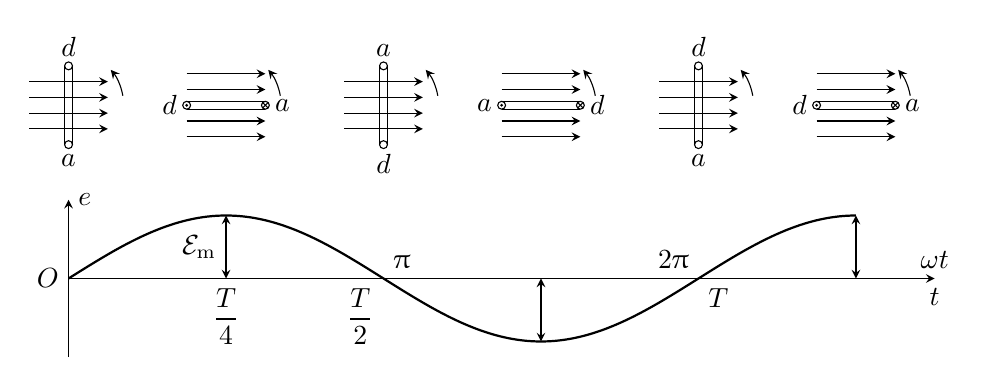
\begin{tikzpicture}[>=stealth, scale=1.0,samples=200]
  \draw [->](0,0)node[left]{$O$}--(11,0)node[below]{$t$};
  \node at (11,0)[above]{$\omega t$};
  \draw [->](0,-1.0)--(0,1.0)node[right]{$e$};
  \draw [thick, domain=0:10]  plot (\x,{0.8*sin(0.25*pi*\x r)});
  \draw[thin,<->](2,0)--(2,{0.8*sin(0.5*pi r)})node[midway,left]{$\mathcal{E}_\text{m}$};
  \draw[thin,<->](6,0)--(6,{0.8*sin(1.5*pi r)});
  \draw[thin,<->](10,0)--(10,{0.8*sin(2.5*pi r)});
  \node at (2,0) [below]{$\dfrac{T}{4}$};
  \node at (4,0) [below left]{$\dfrac{T}{2}$};
  \node at (4,0) [above right]{$\uppi$};
  \node at (8,0) [below right]{$T$};
  \node at (8,0) [above left]{$2\uppi$};
  \begin{scope}[yshift=2.2cm]
    \foreach \x/\t/\b in {0/d/a,4/a/d,8/d/a}
    {
      \foreach \y in {-0.3,-0.1,0.1,0.3}
      {
        \draw[thin,->](\x-0.5,\y)--++(1.0,0);
      }
      \draw(\x,0.5)circle(0.05)node[above]{$\t$}(\x,-0.5)circle(0.05)node[below]{$\b$};
      \draw[->]([shift=(10:0.7)]\x,0)arc(10:40:0.7);
      \draw(\x-0.05,0.5)--++(0,-1);
      \draw(\x+0.05,0.5)--++(0,-1);
    }
    \foreach \x/\l/\r in {2/d/a,6/a/d,10/d/a}
    {
      \foreach \y in {-0.4,-0.2,0.2,0.4}
      {
        \draw[thin,->](\x-0.5,\y)--++(1.0,0);
      }
      \draw(\x-0.5,0)circle(0.05)node[left]{$\l$}(\x+0.5,0)circle(0.05)node[right]{$\r$};
      \fill(\x-0.5,0)circle(0.02);
      \draw(\x+0.5,0)--++(45:0.05)(\x+0.5,0)--++(-45:0.05)(\x+0.5,0)--++(135:0.05)(\x+0.5,0)--++(-135:0.05);
      \draw[->]([shift=(10:0.7)]\x,0)arc(10:40:0.7);
      \draw(\x-0.5,0.05)--++(1,0);
      \draw(\x-0.5,-0.05)--++(1,0);
    }
  \end{scope}
\end{tikzpicture}
\end{document}